\section{Local-view Programming}

\subsection{Introduction}

The user uses Coarray in the local-view model to describe one-sided
communication. In XMP, put/get communication and some synchronization
functions are supported.

If the target system supports Remote Direct Memory Access(RDMA) in the
hardware, one-sided communication in the local-view model can achieve
better performance compared to the global-view model. However, it
requires more effort to describe parallel program since all
communication should be specified in detail.

XMP/Fortran supports Coarray in the standard Fortran 2008. Coarray in
XMP/C has its own original syntax since the C language does not support
Coarray.

\noindent\hrulefill

\noindent {\bf Note}: XMP/Fortran has upward compatibility with Fortran
2008.

\noindent\hrulefill

The basic unit of execution in the local-view is called “image” while it
is called “node” in the global-view model. The two words have the same
meaning in XMP.

\subsection{Coarray Declaration}

\begin{XCexample}
int a[10]:[*];
\end{XCexample}

\begin{XFexample}
integer a(10)[*]
\end{XFexample}

In XMP/C, the user declares a Coarray by adding :[] (Coarray dimension)
after the array declaration. In XMP/Fortran, the user declares a Coarray
by adding [] after the array declaration. The asterisk symbol is used in
both languages.

\noindent\hrulefill

\noindent {\bf Note}: Based on Fortran 2008, the Coarray should have the
same size of the entire execution node group.

\noindent\hrulefill

Coarray can be accessed from other images using assignment
statements. Of course, coarray can be also accessed from your image like
ordinary array.

\subsection{One-sided Communication}

\subsubsection{Put Communication}

When the Coarray reference appears in the left-hand side in an
assignment statement, it causes put communication.

\begin{XCexample}
int a[10]:[*], b[10];

if (xmpc_this_image() == 0)
  a[0:3]:[1] = b[3:3];
\end{XCexample}

\begin{XFexample}
integer a(10)[*]
integer b(10)

if (this_image() == 1) then
  a(1:3)[2] = b(3:5)
end if
\end{XFexample}

The integer number in the Coarray dimension specifies the targer
image. Each image index starts with 0 in XMP/C and starts with 1 in
XMP/Fortran. \|xmpc_this_image()| in XMP/C and \|this_image()| XMP/Fortran
return the current image index.

\noindent\hrulefill

\noindent {\bf Note}: In XMP/Fortran, image index starts with 1 while it
uses [] (similar to C 
style for array dimension) to specify Coarray dimension based on the
standard Fortran 2008.

\noindent\hrulefill

\noindent\hrulefill

\noindent {\bf Note}: When Coarray dimension appears on both side, 3
nodes (target, source, current node) involve the communication.

\noindent\hrulefill

In the above example, XMP/C puts b[3:3] on image 0 to a[0:3] on image
1. XMP/Fortran puts b(3:5) on image 1 to a(1:3) on image 2. The
following figure illustrates the one-sided communication done by
Corray.

\begin{figure}
  \centering
  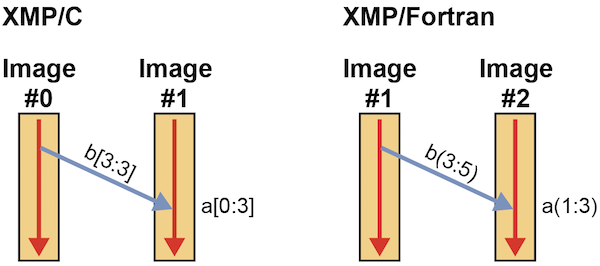
\includegraphics{figs/put.png}
\end{figure}

\noindent\hrulefill

\noindent {\bf Note}: The directives in the global-view model invoke
point-to-point
communication. On the other hand, Coarrays in the local-view model
invoke one-sided communication.

\noindent\hrulefill

\subsubsection{Get Communication}

When a Coarray appears in the right-hand side in the assignment
statement, it causes get communication.

\begin{XCexample}
int a[10]:[*], b[10];

if (xmpc_this_image() == 0)
  b[3:3] = a[0:3]:[1];
\end{XCexample}

\begin{XFexample}
integer a(10)[*]
integer b(10)

if (this_image() == 1) then
  b(3:5) = a(1:3)[2]
end if
\end{XFexample}

In the above program, XMP/C gets a[0:3] from image 1 and stores them on
b[3:3] of image 0. XMP/Fortran gets a(1:3) from image 2 and stores them
on b(3:5) of image 1. The following figure illustrates Coarray get
communication.

\begin{figure}
  \centering
  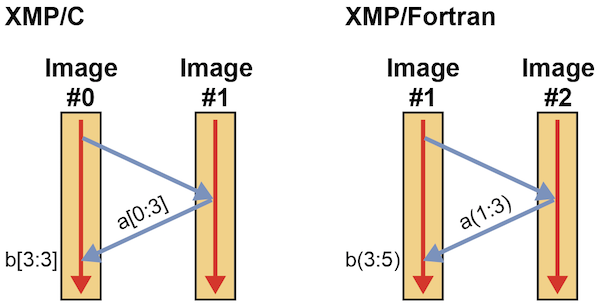
\includegraphics{figs/get.png}
\end{figure}

Hint

As illustrated get needs an extra step to send a request to the target
node. Put communication achieves better performance than get since there
is no such extra step.

\subsubsection{Synchronization}

Here, we introduce “sync all” which is most frequently used among
Coarray synchronization functions.

\begin{XCexample}
void xmp_sync_all(int *status)
\end{XCexample}

\begin{XFexample}
sync all
\end{XFexample}

The “sync all” waits all issued one-sided communication and invokes
barrier synchronization among the entire images.

\begin{figure}
  \centering
  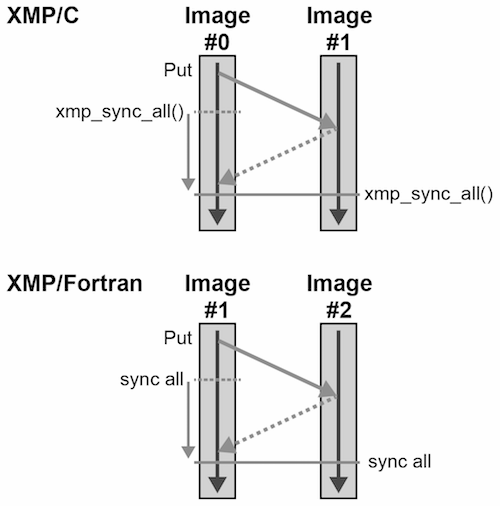
\includegraphics{figs/sync_all.png}
\end{figure}

In the above example, the left image puts data to the right image and
both nodes invoke sync all. When both nodes finish sync all, the
execution continues after the synchronization point.

% 3.5. Tutorial
% Run the following sample using 2 images.

% XMP/C program
% #include <stdio.h>
% #include <xmp.h>
% int a[10]:[*], b[10]:[*], c[10][10]:[*];

% int main(){
%   int me = xmpc_this_image();

%   for(int i=0;i<10;i++)
%     a[i] = b[i] = i + 10 * me;

%   for(int i=0;i<10;i++)
%     for(int j=0;j<10;j++)
%       c[i][j] = (i * 10 + j) + 100 * me;

%   xmp_sync_all(NULL);

%   if(xmpc_this_image() == 0){
%     a[0:3] = a[5:3]:[1];            // Get
%     for(int i=0;i<10;i++)
%       printf("%d\n", a[i]);

%     b[0:5:2] = b[0:5:2]:[1];       // Get
%     printf("\n");
%     for(int i=0;i<10;i++)
%       printf("%d\n", b[i]);

%     c[0:5][0:5]:[1] = c[0:5][0:5]; // Put
%   }
%   xmp_sync_all(NULL);

%   if(xmpc_this_image() == 1){
%     printf("\n");
%     for(int i=0;i<10;i++){
%       for(int j=0;j<10;j++){
%       printf("  %3d",c[i][j]);
%       }
%       printf("\n");
%     }
%   }

%   return 0;
% }
% XMP/Fortran program
% program main
%   implicit none
%   include "xmp_coarray.h"
%   integer :: a(10)[*], b(10)[*], c(10,10)[*]
%   integer :: i, j, me

%   me = this_image()

%   do i=1, 10
%     b(i) = (i-1) + 10 * (me - 1)
%     a(i) = b(i)
%   end do

%   do i=1, 10
%     do j=1, 10
%       c(j,i) = ((i-1) * 10 + (j-1)) + 100 * (me - 1)
%     end do
%   end do

%   sync all

%   if (this_image() == 1) then
%     a(1:3) = a(6:8)[2] ! Get
%     do i=1, 10
%       write(*,*) a(i)
%     end do

%     b(1:10:2) = b(1:10:2)[2];  ! Get
%     write(*,*) ""
%     do i=1, 10
%       write(*,*) b(i)
%     end do

%     c(1:5,1:5)[2] = c(1:5,1:5) ! Put
%   end if

%   sync all

%   if (this_image() == 2) then
%     write(*,*) ""
%     do i=1, 10
%       write(*,*) c(:,i)
%     end do
%   end if
% end program main
% In the above example, 3 Coarrays a, b, c are declared. a and b are 1-dimensional arrays and c is a 2-dimensional array. The following shows the initial values of each array.

% Image 0 in XMP/C, Image 1 in XMP/Fortran
% a : from 0 to 9
% b : from 0 to 9
% c : from 0 to 99
% Image 1 in XMP/C, Image 2 in XMP/Fortran
% a : from 10 to 19
% b : from 10 to 19
% c : from 100 to 199
% 3.5.1. One-sided communication for contiguous region
% In the first get communication, in XMP/C, image 0 gets a[5:3] from image 1 and stores them to a[0:3]. In XMP/Fortran, image 1 gets a[6:8] from image 2 and stores them to a(1:3)

% After the communication, array a has the following values.

% 15
% 16
% 17
% 3
% 4
% 5
% 6
% 7
% 8
% 9
% 3.5.2. One-sided communication for discontiguous region
% In the second get communication, in XMP/C, image 0 gets b[0:5:2] from image 1 and stores them to b[0:5:2]. In XMP/Fortran, image 1 gets b(1:10:2) from image 2 and stores them to b(1:10:2).

% After the communication, array b has the following values.

% 10
% 1
% 12
% 3
% 14
% 5
% 16
% 7
% 18
% 9
% 3.5.3. One-sided communication for multi-dimensional array
% In the put communication, in XMP/C, image 0 puts c[0:5][0:5] to on c[0:5][0:5] image 1. In XMP/Fortran, image 1 puts c(1:5,1:5) to c(1:5,1:5) on image 2. The communication has the block-strided communication pattern.

% After the communication, array c has the following values.

%   0    1    2    3    4  105  106  107  108  109
%  10   11   12   13   14  115  116  117  118  119
%  20   21   22   23   24  125  126  127  128  129
%  30   31   32   33   34  135  136  137  138  139
%  40   41   42   43   44  145  146  147  148  149
% 150  151  152  153  154  155  156  157  158  159
% 160  161  162  163  164  165  166  167  168  169
% 170  171  172  173  174  175  176  177  178  179
% 180  181  182  183  184  185  186  187  188  189
% 190  191  192  193  194  195  196  197  198  199


\subsection{Synchronization Statements}

\subsubsection{sync all}

\begin{XCexample}
void xmp_sync_all(int *status)
\end{XCexample}

\begin{XFexample}
sync all
\end{XFexample}

Barrier synchronization is performed among all images after completing
all one side communications. For details, see Tutorial (Local-view).

\subsubsection{sync images}

\begin{XCexample}
void xmp_sync_images(int num, int *image-set, int *status)
\end{XCexample}

\begin{XFexample}
sync images (image-set)
\end{XFexample}

Barrier synchronization is performed among the specified images after
completing all one side communications.

\begin{XCexample}
int image_set[3] = {0,1,2};
xmp_sync_images(3, image_set, NULL);
\end{XCexample}

\begin{XFexample}
integer :: image_set(3) = (/ 1, 2, 3/)
sync images (image_set)
\end{XFexample}

\subsubsection{sync memory}

\begin{XCexample}
void xmp_sync_memory(int *status)
\end{XCexample}

\begin{XFexample}
sync memory
\end{XFexample}

Wait for completion of all one side communications. This function does
not include barrier synchronization unlike sync all and sync images, so
it is executed only locally.

% 20.2. Arguments

% XMP/C program
% void xmp_sync_all(int *status)
% void xmp_sync_images(int *status)
% void xmp_sync_memory(int *status)

% XMP/Fortran program
% sync all [stat=..] [errmsg=..]
% sync images (image-set) [stat=..] [errmsg=..]
% sync memory [stat=..] [errmsg=..]

% In XMP/C, if synchronization is successful, “XMP_STAT_SUCCESS” which is
% the constant defined in xmp.h is assigned to status. If any images have
% already ended, “XMP_STAT_STOPPED_IMAGE” is substituted to status. In
% case of other errors, a value other than the above two values is
% assigned to status.

% Similarly, if synchronization is successful in XMP/Fortran,
% “STAT_STOPPED_IMAGE” is assigned to the variable on the right-hand side
% of stat=, and if any images have already ended, “STAT_STOPPED_IMAGE” is
% assigned. In case of other errors, a value other than the above two
% values is assigned.

% Hint

% In XMP/Fortran, if you omit stat= and errmsg=, synchronization speed
% will be faster. In XMP/C, assignment of status can be omitted by using
% NULL like xmp_sync_all (NULL);

\subsection{{\tt post}/{\tt wait} Construct}

\subsection{{\tt lock}/{\tt unlock} Construct}

